\chapter{Background}
\label{chp:background} 

\todo{ingress}

\section{Side-channels}\label{chp2:sec:side_channel}
Side-channel attacks is not the kind of standard attack like brute-force attack where you try every single combination to crack a cryptographic algorithm, or like a theoretical weakness that you can take advantage of in cryptographic implementations. 
Side-channel attack exploits the physical implementation to gain information about a cryptographic system.
Characteristics a side-channel attack might exploit can be the power consumption, timing information, electromagnetic radiation, information obtained from a storage after deletion or even sound leakage from the target machine.

%Covert-channel attack allows the adversary to communicate with two objects in a physical matter that is not supposed to be allowed. 
%An attack like this is useful when the adversary is able to get inside a computer, but not able to communicate with others what he finds. 
%If the adversary knows about a channel, he can use this to transfer the knowledge he has learned.
%This channel can be a hardware device that is apparently leaking sound in a frequency that humans cannot hear.


\subsection{Acoustic cryptanalysis}\label{chp2:subsec:acoustic_cryptanalysis}

Acoustic cryptanalysis is done by listening to sound that is emitted by computers. 
Computers leaks sound from Hz to several hundred kHz. 
\todo{Write something more.. general stuff about acoustic cryptanalysis}

In 2005, some researchers at Berkeley did a research~\cite{url:keystrokes} on recognizing keystrokes on a keyboard by sound. 
This is possible because each key has its own distinct sound. 
After separating the different keystrokes, they used a statistical frequency method to find out which key belonged to which letter. 
To determine the letters, they only had to listen for 10 minutes, i.e. on a typical user that types about 300 characters each minute. 
One method to take advantage of this attack is to create a mobile phone application that enables the microphone and analyses the keystrokes. 

Its also proven that phones and ATMs with mechanical keyboards can be vulnerable for acoustic attacks~\cite{DBLP:conf/sp/AsonovA04}.

In 2014, a research team at the Tel Aviv University was able to do a full RSA Key (4096-bit) extraction using acoustic cryptanalysis. 
This research is explained in more detail in~\autoref{chp2:subsec:original_research}.

\subsection{Data remanence}\label{chp2:subsec:data_remanence}

Data remanence is remaining representation if digital bits after attempts of deletion or removal of data. 
The recovery of these bits may be due to the technique used to delete or the physical characteristics of the storage media. 
The problem of data remanence was first observed in magnetic media, when it was proven that data could be restored after several times of overwriting. 
Earlier it has been shown that for some UV EPROM, EEPROM and Flash devices, information can still be recovered after 100 erase cycles\cite{DBLP:conf/ches/Skorobogatov05}.
These proofs is however just theoretical proofs. 
Nobody has proven in practice to restore bits after been overwritten. 

\subsection{Differential fault analysis}\label{chp2:subsec:differential_fault_analysis}

Differential fault analysis is cryptanalysis based on interpreting fault outputs from a processor exposed to different kinds of environmental exposure like high voltage or current, strong electromagnetic fields or as simple as high temperature. 
The processor might give fault outputs an adversary can use to find knowledge about the processor state or similar information.


Guo, et al (2013): Invariance-based concurrent error detection for advanced encryption standard~\cite{DBLP:journals/iacr/GuoK13}
\todo{Is this paper something to write about?}

Giraud (2003): DFA on AES~\cite{DBLP:journals/iacr/Giraud03}
\todo{Is this paper something to write about?}

\subsection{Electromagnetic attacks}\label{chp2:subsec:electromagnetic_attacks}

An adversary can, if located within range, intercept electromagnetic signal emitted by all electronic devices. 
It is not possible to detect this attack, and therefore hard to prevent. 
One of the known attacks is extracting the electromagnetic signals from a computer monitor to reproduce the screen output.
These signals originates from the electron gun that manipulates each pixel~\cite{url:tempest_sans}. 
The stronger a pixel is, the stronger the signal.
PGP includes a secure viewer that prevents exactly these high frequency signals by making softened edges in the fonts.
However, it is said to be very difficult, thus expensive to extract the signals emitted by a computer monitor. 

\subsection{Power analysis}\label{chp2:subsec:power_analysis}

Electronic devices leaks information about what they are processing through their power consumption.
This leakage can be used to extract secret information like keys used to encryption using differential power analysis (DPA). 

Simple power analysis (SPA) is simply interpreting the power consumption measurements during cryptographic operations~\cite{DBLP:conf/crypto/KocherJJ99}. 

DPA is a more complex way to interpret the power consumption. \todo{write something fancy about DPA}
Paul Kocher: Differential power analysis~\cite{DBLP:conf/crypto/KocherJJ99}

\subsection{Timing attacks}\label{chp2:subsec:timing_attacks}

Here goes related work to timing attacks

SSL Timing attack~\cite{DBLP:conf/esorics/BrumleyT11}
Timing attack Diffie-Hellman~\cite{DBLP:conf/crypto/Kocher96}


\section{Related work}\label{chp2:sec:related_work}

The research done in the area of acoustic emanations from a computer is limited. 

\subsection{Original research - Acoustic Cryptanalysis}\label{chp2:subsec:original_research}

We base our project on a work done by some Israeli researchers, Daniel Genkin, Adi Shamir and Eran Tromer.
The research they have done is the RSA Key Extraction via Low-Bandwidth Acoustic Cryptanalysis~\cite{DBLP:conf/crypto/GenkinST14}.
Their claim is that many computers leaks acoustic noise from its electronic components due to vibration, i.e. coil whine (noise).
Vital components like the CPU requires power dependent on what it is computing.
Hence the theory is that some CPUs leaks acoustic noise about what it is doing.
They use this information to extract a 4096-bit RSA key.

\subsubsection*{Lab setup}\label{chp2:subsubsec:lab_setup}

The noise they are trying to record and interpret is found in different and high frequencies, thus high sensitivity microphones is required. 
They use 3 different microphones from Brüel\&Kjær showed in figure~\ref{fig:bruel_kjaer_mics}

\begin{figure}[h]
	\centering
    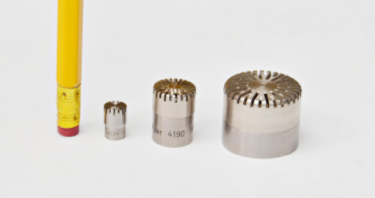
\includegraphics[width=0.4\textwidth]{bruel_kjaer_mics.png}
    \caption{Brüel\&Kjær 4145 (up to 21kHz), 4190 (up to 40kHz) and 4939 (up to 350kHz)~\cite{DBLP:conf/crypto/GenkinST14}.}
    \label{fig:bruel_kjaer_mics}
\end{figure}


\subsubsection*{Acoustic leakage}\label{chp2:subsubsec:acustic_leakage}


\subsubsection*{RSA key extraction}\label{chp2:subsubsec:rsa_key_extraction}

